\documentclass[english,12pt,a4paper]{book}
%TODO: Correct format, not a4
\usepackage[T1]{fontenc} % In case we want special characters
\usepackage[utf8]{inputenc} % We are all writing in UTF-8

\usepackage[numbers]{natbib} % We need to tweak our referencing a bit.
\usepackage{appendix} % Fixes formatting of appendices
\usepackage[printonlyused]{acronym} % Package to handle the acronym list
\usepackage{graphicx} % We *may* use images
\graphicspath{{images/}} % and it is clean to put them in a separate dir
\usepackage{hyperref} % Internal and external links is nice
\hypersetup{pdfborder=0 0 0} % ..especially without red borders
\usepackage{amstext} % To support \text in math mode

% Packages and settings for code listings
\usepackage{listings}
\usepackage{caption}
\usepackage{upquote}
\usepackage{xcolor}
\DeclareCaptionFont{white}{\color{white}}
\DeclareCaptionFormat{listing}{\colorbox{gray}{\parbox{\textwidth}{#1#2#3}}}
\captionsetup[lstlisting]{format=listing,labelfont=white,textfont=white}
\lstset{
language=Java,
keywordstyle=\bfseries\ttfamily\color[rgb]{0,0,1},
identifierstyle=\ttfamily,
commentstyle=\color[rgb]{0.133,0.545,0.133},
stringstyle=\ttfamily\color[rgb]{0.627,0.126,0.941},
showstringspaces=false,
basicstyle=\small,
numberstyle=\footnotesize,
numbers=left,
stepnumber=1,
numbersep=10pt,
tabsize=2,
breaklines=true,
prebreak = \raisebox{0ex}[0ex][0ex]{\ensuremath{\hookleftarrow}},
breakatwhitespace=false,
aboveskip={1.5\baselineskip},
columns=fixed,
upquote=true,
extendedchars=true,
frame=bottomline,
inputencoding=utf8
}

% Set equal margins on book style
% \usepackage{layout} % Use \layout to print out the margins (debug)
\usepackage{geometry}
\geometry{bindingoffset=1cm}

% Restyle chapter headers
\usepackage{fix-cm}
\makeatletter
\renewcommand{\@makechapterhead}[1]{%
  \vspace*{50\p@}%
  {\parindent \z@ \raggedright \normalfont
    \vspace{15pt}%
    \ifnum \c@secnumdepth >\m@ne
        %\hfill\huge\scshape \@chapapp\space
        \hfill\fontsize{60}{90}\selectfont \thechapter % Chapter number
        \par\nobreak
        \vskip 20\p@
    \fi
    \interlinepenalty\@M
    \hfill \Huge \scshape #1\par % Chapter title
    \vspace{5pt}
    \hrule
    \nobreak
    \vskip 40\p@
  }}
\makeatother

\author{Eirik Haver \and Eivind Melvold \and Pål Ruud}
\title{Master thesis - Cloud Storage Vault}
\date{\today}

\begin{document}

\include{title}
\pagestyle{empty}

\chapter*{Abstract}
\addcontentsline{toc}{chapter}{Abstract}
\pagestyle{plain}
\pagenumbering{Roman}
\setcounter{page}{1}

%  Writers should follow a checklist consisting of:
% Motivation: Why do we care about the problem and results?
% Problem Statement: What problem are we trying to solve? Scope/limits.
% Approach: How did we go about solving or making progress on the problem?
% Results: What is the answer? Numbers, not vague 'very', 'small' etc.
% Conclusions: What are the implications of your answer? Further work.
%
%  Each section is typically a single sentence, although there is room for
%  creativity.

\chapter*{Preface}
\addcontentsline{toc}{chapter}{Preface}

The work behind this project report was carried out during the spring semester
in 2011 at the Norwegian University of Science and Technology (NTNU), Department
of Telematics (ITEM).
\vspace{13pt}

\begin{center}
Eirik Haver, Eivind Melvold and Pål Ruud
\vspace{13pt}

\end{center}

\tableofcontents

\cleardoublepage
\phantomsection
\addcontentsline{toc}{chapter}{\listfigurename}
\listoffigures

\cleardoublepage
\phantomsection
\addcontentsline{toc}{chapter}{\listtablename}
\listoftables

\cleardoublepage
\phantomsection
\addcontentsline{toc}{chapter}{\lstlistlistingname}
\lstlistoflistings
\cleardoublepage

\chapter*{Acronyms}
\addcontentsline{toc}{chapter}{Acronyms}

\begin{acronym}
\acro{ACL}{Access Control List}
\acro{AES}{Advanced Encryption Standard}
\acro{CA}{Certification authority}
\acro{DSA}{Digital Signature Algorithm}
\acro{DSS}{Digital Signature Scheme}
\acro{FAQ}{Frequently Asked Questions}
\acro{IaaS}{Infrastructure as a Service}
\acro{LAFS}{Least Authority File System}
\acro{MITM}{Man-in-the-middle}
\acro{NIST}{National Institute of Standards and Technology}
\acro{PBKDF2}{Password-Based Key Derivation Function version 2}
\acro{PaaS}{Platform as a Service}
\acro{PGP}{Pretty Good Privacy}
\acro{PKI}{Public Key Infrastructure}
\acro{RSA}{Rivest, Shamir and Adleman}
\acro{SaaS}{Software as a Service}
\acro{SHA}{Secure Hash Algorithm}
\acro{SSL}{Secure Socket Layer}
\acro{TLS}{Transport Layer Security}
\acro{VM}{Virtual Machine}
\end{acronym}

%**************************************%
\chapter{Introduction}
%**************************************%
\pagenumbering{arabic}
\setcounter{page}{1}

\section{Method}

\section{Outline}

The work is presented as per the following chapters:

\paragraph{Chapter 2} provides background knowledge of the technologies and
software used.


%**************************************%
\chapter{Background}
%**************************************%
% Cloud (computing)
\section{Security Services}
This section briefly explains certain security services used in this
thesis. A security service is any processing or communication service that
enhances the security of the data processing systems and the information
transfers of any organization\cite[p. 12]{stallings}.

\paragraph{Confidentiality} is the art of keeping a message secret from
unauthorized parties\cite[p. 18]{stallings}. This can typically be done by
either preventing other parties access to the message at all, or making the
contents unreadable for instance by the use of encryption. 

\paragraph{Integrity} in a security perspective deals with detecting,
preventing or recovering a message from being changes by an unauthorized party
\cite{stallings}.

\paragraph{Authentication} is the act for a user, service or similar to prove
that he is what he claims to be\cite{stallings}. 

\subsection{Nonrepudiation} prevents either sender or receiver of a message
from denying a transmitted message, in other words one party can prove the
other parties involvement\cite{stallings}.

\section{Cryptographic Primitives}
This section explains the low level security primitives used in this thesis.

\subsection{Encryption}
Encryption is the process of transforming some information into an unreadable
form. Encryption is primarily used to enforce Confidentially, but can also be
used for other purposes such as authentication. In a very basic form an
encryption scheme consist of an algorithm, the cipher, a key and a message, the
plaintext, that is all used to create an encrypted message, a ciphertext. If
a good cipher is used, knowledge of the cipher, plaintext and ciphertext should
not be enough to obtain the key.

\paragraph{Block-cipher and Stream-cipher} are classifications on how a cipher
treats data\cite[p. 32]{stallings}. With a block-cipher data will be encrypted
in blocks of specific sizes. If the data length is not a multiple of the block
size, the data will be padded. A stream cipher on the other hand will encrypt
the message co.

\paragraph{Symmetric encryption} is an encryption scheme where the same key is
used for both encryption and decryption\cite[p. 32]{stallings}. \ac{AES} is a
block cipher and is the current standard for symmetric encryption. \ac{AES}
works on a block of 128-bit and support keys of 128, 192 and 256-bit. 

\paragraph{The mode of operation} used for a symmetric encryption scheme
enables subsequent safe use of the same key.
%TODO: Vi kan ikke nevne alle her, vi nevner de som er nødvendige. CBC?

\paragraph{Asymmetric encryption} is an encryption scheme where a different key
is used for encryption than decryption\cite[p. 259]{stallings}. An asymmetric
encryption scheme is often called a public-key encryption scheme, where one key
is defined as private and the other as public. The public key is shared to
allow other parties to encrypt messages for the owner of the private key. The
downside of asymmetric encryption compared to symmetric is that it requires a
larger key and has a larger computational overhead to obtain the same level of
confidentiality. The probably best known asymmetric cipher is \ac{RSA}.

\subsection{Cryptographic hash functions}
A cryptographic hash function is a deterministic mathematical procedure which
takes an arbitrary block of data and outputs a fixed-size bit string. The output
is referred to as the hash value, message digest or simply digest.
Another property of a cryptographic hash function is that the smallest change in
the input data (e.g. one bit) should completely change the output of the hash
function. In other words it should be infeasible to find the reverse of a
cryptographic hash function \cite[p. 335]{stallings}. It should also be infeasible to
find two blocks of data which produce the same hash value (a \emph{collision}).

The standard for cryptographic hash functions today are \ac{SHA}-1 and the
\ac{SHA}-2 family.

\section{Applications of cryptographic primitives}

\subsection{Digital Signatures}
A digital signature is the digital equivalent of a normal signature, it
verifies that an entity approves with or has written a message, the date the
signature was made and it should be verifiable by a third party \cite[p.
379]{stallings}. It should logically not be possible or at least unfeasible to
fake a digital signature. It is possible to create digital signatures with
\ac{RSA} there is also a standard for digital signatures called \ac{DSS} which
uses \ac{DSA} as the actual algorithm.

\subsection{Digital Certificates and PKI} A digital certificate is the pairing
of a digital signature and a public key\cite{stallings}.  By this scheme the
services confidentiality, authentication and nonrepudiation can be achieved.
Basically a person or other entity has a certificate with some clues about the
identity in it, e.g. the e-mail, together with a public key. This certificate
can then be signed using digital signatures to verify that some other entity
trusts this certificate. In practise the entity which signs certificates is the
\ac{CA} which all clients have the public key information for, and trusts. The
\ac{CA} will also contain information about which certificates has been
revoked, i.e. should not be trusted in use. Such a scheme is usually referred
to as a \ac{PKI}.

\subsubsection{PGP} \ac{PGP} is a scheme similar to \ac{PKI} but with no
\ac{CA} that all users trusts\cite{stallings}. Instead trust is made between
users by somehow verifying their public key, for instance by meeting face to
face. A user can then sign another users key, set a trust level for the user
and publish this information to a keyserver. Another user can then calculate a
trust to an unknown person based on the trust set by peoples that he trusts. 

\subsection{SSL/TLS}
\ac{TLS} and its predecessor \ac{SSL} are techniques for obtaining
confidentiality, integrity for transfer of files over a
network\cite{stallings}. It does so by a combination of different algorithms
and primitives, but a digital certificate is required for authentication. 

\subsection{PBKDF2}
%TODO: See if we actually use this.
\ac{PBKDF2} is a key derivation function to create an encryption key based on
a password. The point of this is that a password is often something that should
be memorable to a person, but what is memorable to a person might be a to short
phrase to withstand a brute force attack. What \ac{PBKDF2} does is make the
process of deriving the key from the password an expensive process in terms of
computational power, to make it more resistant to brute force attacks.

\section{Security Attacks}
This section briefly list security attacks relevant to this thesis, as defined
by \citeauthor{stallings}.
%TODO: Mulig man skal bruke en annen måte å refere kilden på her

\paragraph{Active and passive attacks} are classifications of security attacks,
where a passive attack attempts to learn or make use of information from the
system but does not affect system resources. An active attack attempts to alter
system resources or affect their operation.

\paragraph{Traffic analysis} is the art of capturing communication sent between
two parties. This information might contain secrets or might for instance leak
enough information about an encryption key to make it breakable. 

\paragraph{Masquerade} is an active attack where the attacker pretends to be
one of the legit parties.

\paragraph{Replay} is an active attack where the attacker capture some data in
a communication session and subsequently retransmit that information.

\paragraph{Modification of messages} is an active attack where the attacker
alters some of the contents of a message sent between two communicating
parties.

\paragraph{Denial of Service} is an active attack where the attacker seeks to
make resources unavailable for legit users, i.e. by overloading an application
by sending it lots of traffic.

\paragraph{\acl{MITM}} is an attack where an attacker intercepts messages
between the communicating parties and then either relay or substitute the
intercepted message.

\subsection{Attacks on cryptographic primitives}
Even though cryptographic primitives are designed to be secure, they might have
both flaws and be used in an incorrect fashion. 

\paragraph{Cryptanalysis attack} is an attempt to deduce a specific plaintext
or to deduce the key being used in a ciphertext.

\paragraph{Brute-force attack} is an attack where you try to obtain a secret by
testing the algorithm with up to all possible inputs. The secret might be an
encryption key or the data fed into a cryptographic hash function.

\section{Cloud Computing} 
In a draft\cite{cloud_nistdef} \ac{NIST} defines cloud computing as:
\begin{quote} 
Cloud computing is a model for enabling ubiquitous, convenient,
on-demand network access to a shared pool of configurable computing resources
(e.g., networks, servers, storage, applications, and services) that can be
rapidly provisioned and released with minimal management effort or service
provider interaction.  
\end{quote}

\subsection{Service Models}
\ac{NIST} also defines three service models which deals with what kind of
service the consumer is able to rent from a provider.

\paragraph{\ac{SaaS}} is the capability for a consumer to run the provider's
application running on cloud infrastructure, using a thin-client, browser or
similar. Gmail\footnote{\url{http://www.gmail.com}} can be seen as an example
of this.

\paragraph{\ac{PaaS}} is the capability for a consumer to deploy software onto
the cloud, but without actually controlling the underlying platform, operating
system etc.

\paragraph{\ac{IaaS}} is the capability provided to the consumer to provision
processing, storage, networks and other fundamental computing resources where
he can run arbitrary software, including operating systems and applications. An
example is hiring a \ac{VM}.

\subsection{Deployment Models}
The \ac{NIST} draft also lists several Deployment Models which deals with how
the cloud is organized in terms of where it is hosted and who has access to it.

\paragraph{Private Cloud} is a cloud infrastructure operated solely for an
organization. Which party manages the cloud and where it is located is not
given.

\paragraph{Community Cloud} is a cloud infrastructure is shared by several
organizations to serve a common concern. Where it is located and who manages it
is not given.

\paragraph{Public Cloud} is a cloud infrastructure where basically everyone or
at least a large group can have access, and is owned by a external provider of
cloud services.

\paragraph{Hybrid Cloud} is a cloud infrastructure composed of two or more
clouds of any other model. 

\subsection{Security considerations} 
There are some considerations when using cloud services from an external provider 
as opposed to self controlled hardware, software and plattforms. Most notably
is that you loose the control of selecting the people which will have physical
and digital access to the infrastructure. In essence this means that the
provider can read every data sent to and from the cloud as well as the data
saved in the cloud.

Another risk is that information might be leaked to other users of the same
cloud. For instance it might be able possible for a \ac{VM} to leak information
to other \ac{VM}s on the same host. 
%TODO: kilde

\section{Existing Solutions}
There are a number of existing storage solutions for storing data in the cloud,
with more or less of the functionality required to fulfill the problem
description for this thesis. The section highlights some of them.

\subsection{Dropbox} Dropbox\footnote{\url{http://www.dropbox.com}} is a
commercial application for storing data in the cloud, more specific using
Amazons S3 storage service. It claims that files are stored encrypted with
\ac{AES}-256 which can only be decrypted with the users username and password,
and that Dropbox employees are not able to access the files of the
user\footnote{\url{http://www.dropbox.com/help/27}}. However Dropbox also has a
Forgot password feature which means that Dropbox can read the users files if
they really want to. Their \ac{FAQ} does however say that some people have been
successfull in putting truecrypt containers in Dropbox which effectivly makes
dropbox secure\footnote{\url{http://www.dropbox.com/help/179}}.

\subsection{Tahoe-LAFS}
Tahoe-\ac{LAFS}\footnote{http://www.tahoe-lafs.org} is an open source
cloud storage file system which does fulfill the requirements set by our
problem description in regards to security. In Tahoe-\ac{LAFS} files are
exclusivly encrypted client-side, before beeing uploaded into the cloud.
Tahoe-\ac{LAFS} also uses erasure-coding to obtain redundancy across multiple
storage servers.  

%TODO: kilde, enten paperet vi brukte i prosjektet, muligens
% http://tahoe-lafs.org/source/tahoe-lafs/trunk/docs/about.html

%**************************************%
\chapter{Architectural Solution}
%**************************************%
\label{chap:AS}

The architectural solution of a secure cloud file sharing system has to convince
its users that the functions indeed are secure, and that the concepts are easy
to understand and accept.

\section{Introduction}
% FIXME: Can we just drop this section and include its contents in the chapter
% intro?

The architecture has to support various user functionality. Figure
\ref{fig:arch:overview} exhibits Alice uploading files to the cloud, and
thereafter transferring the necessary information to Bob so that he also can
gain access to the files.

\begin{figure}[h!]
    \centering
    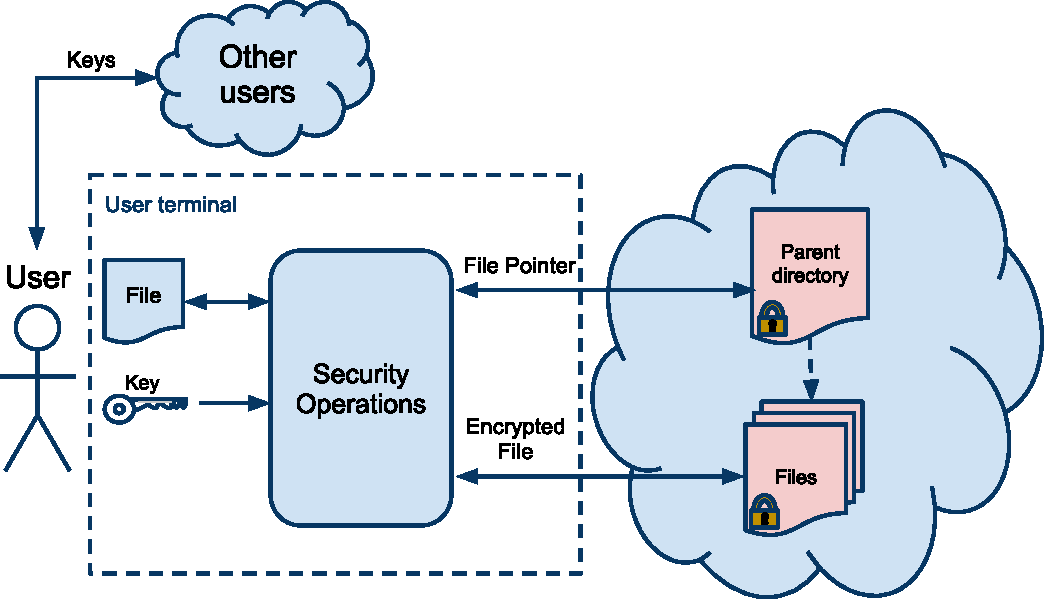
\includegraphics[width=\columnwidth]{ArchitectureOverview.pdf}
    \caption{Overview of user functionality}
    \label{fig:arch:overview}
\end{figure}

In the following sections, we will describe how the file storage is organized,
and take a closer look at how the different functionality are solved.

\section{File Storage}
\label{sec:AS:FS}

The solution proposed in this thesis, is that only a simple key-value store is
needed on the server side. This may be extended with an \ac{ACL} layer to
support user access and other features.

Two types of files exist: immutable and mutable files. The mutable files are used
as directories, in the sense that they contain the information needed to access
other directories or files in the form of capabilities.
A capability is a short alphanumeric string containing all information needed
to find, get, read and write a file or folder. This includes an identifier and
cryptographic keys.

In principle, the only operations the key-value store need to support are
\textbf{PUT}, \textbf{GET} and \textbf{UPDATE}. The latter one is required to
make changes to the ``directory'' files.

% Picture: "Architecture: Directory tree"

% TODO:
% - Various File access modes (RO/RW)

\section{User scenarios}

The various user scenarios the software has to support, provides a logic way to
describe the external properties of the system. The fundamental operations are
\emph{downloading}, \emph{uploading} and \emph{sharing} of files.

\subsection{Download file}

When a user wishes to download a file or directory, all that is needed is the
password to unlock the local keyring on the user terminal, as depicted in Figure
\ref{fig:arch:download}. The client sends a GET request with the identifier in
question, and the server responds with the encrypted folder. This contains the
capabilities needed to locate and decrypt the underlying files and folders.
After decrypting the contents, the client again queries the server with the
identifier of the wanted file, and there after decrypts it, before displaying it
to the user.

\begin{figure}[h!]
    \centering
    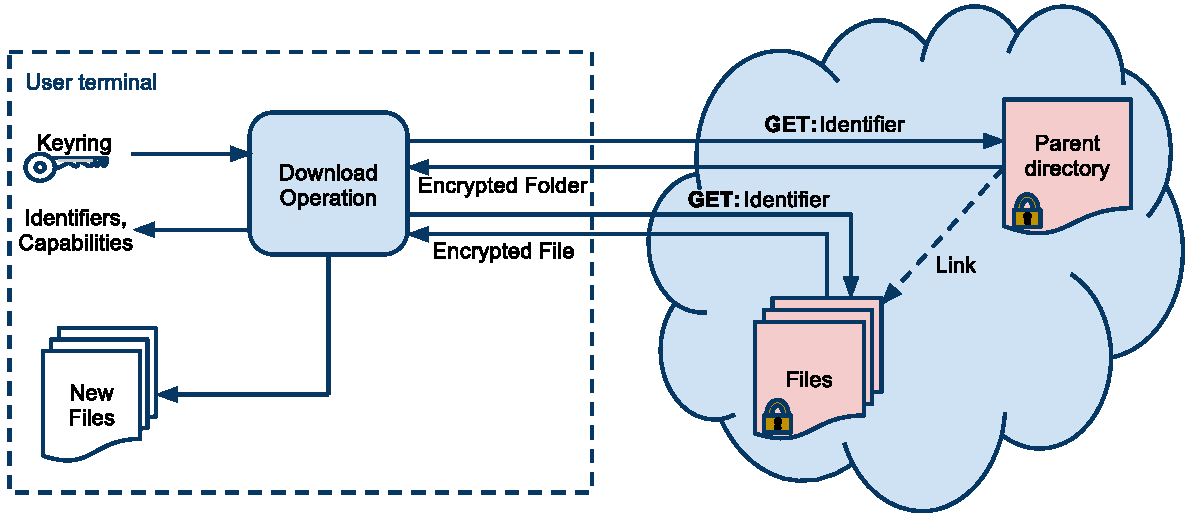
\includegraphics[width=\columnwidth]{ArchitectureDownload.pdf}
    \caption{Scenario: Downloading of files}
    \label{fig:arch:download}
\end{figure}

\subsection{Upload Files}

Figure \ref{fig:arch:upload} shows the process of uploading a new file. The only
information the server in the cloud receives, are identifiers and encrypted
containers. The user is also given the opportunity to transfer the corresponding
identifiers and capabilities to users.

Before uploading, the client has to download and decrypt the directory the
files are to be placed in. This process was described in the previous section.
The cryptographic details of the Upload Operation can be found in Section
\ref{sec:CS:UF}.

\begin{figure}[h!]
    \centering
    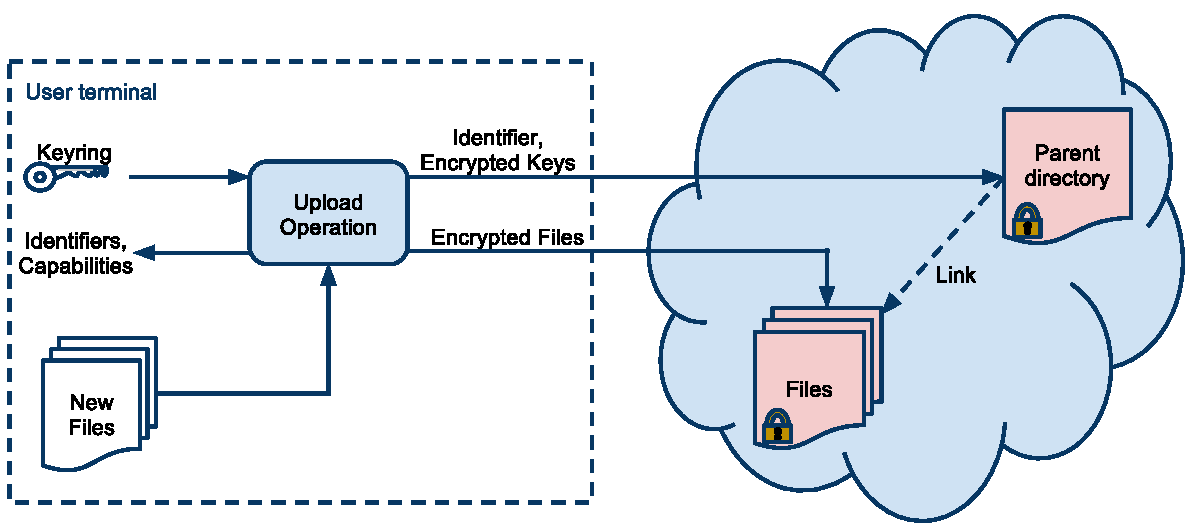
\includegraphics[width=\columnwidth]{ArchitectureUpload.pdf}
    \caption{Scenario: Uploading of files}
    \label{fig:arch:upload}
\end{figure}

\subsection{Share files}


%**************************************%
\chapter{Cryptographic Solutions}
%**************************************%
\label{chap:CS}
This chapter will elaborate on the cryptographic solutions applied to the
architectural scheme in Chapter \ref{chap:AS}. We will take a closer look at
how confidentiality, integrity, authentication and access control can be 
integrated into the proposed architecture.

A fundamental scheme for key distribution is needed to realize the desired
security features, hence an appropriate solution for key distribution will
also be given.

In the first section, we will give a brief introduction explaining the basic security
scheme used in the application. We will further look at each file operation 
exhibited in Chapter \ref{chap:AS} and describe our corresponding cryptographic
solution. The following section will give a detailed overview of the
cryptographic keys used in the mentioned file operations. The chapter will end with an 
explanation of the chosen scheme for key distribution.

\section{Basic Security Scheme}
The basic security concept of our application is to keep a users remote storage
confidential to a third-party storage provider. To solve this, we will
create an application that encrypt files locally at the users terminal before
they are uploaded to the third-party storage provider. To further access files, the user will have
to decrypt files locally when downloading them. To enable this simple
encryption scheme, the user is required to possess at least one cryptographic key.

By initially knowing that files are encrypted on a remote server and that the local user
possess one or more cryptographic keys, we can continue with a more comprehensive
description of the complete cryptographic solution. The details of the complete
solution will be explained in the manner of 3 different file operations, namely
upload, download and share file.

\section{Upload File}
\label{sec:CS:UF}
The process of uploading a file onto a network server was illustrated in Figure
\ref{fig:U}. This section will provide a more detailed description of the
process and specify the functionality of the Upload operation at the user
terminal.

The upload process can be broken into the following 5 steps:

\begin{enumerate}
\item Download and decrypt parent directory to target file
\item Generate file keys and capabilities
\item Write file meta data to parent directory
\item Encrypt and upload directory
\item Encrypt and upload file
\end{enumerate}

Each step is described below.

\subsection{Download and Decrypt Directory}
When uploading a file to the remote file structure described in \#\#, two
operations are needed. First of all, it is important to add the desired file's
meta data into the remote parent directory. This meta data will serve as a link
to the uploaded file. The second operation is to upload the desired file.

To insert the file's meta data into the remote directory, it is necessary to
download and decrypt the chosen directory. We will combine the download and
decrypt procedures into the term ``open directory''. The procedure of opening a
directory is illustrated in Figure \ref{fig:OD} and described as follows.

%\begin{figure}[h!]
%    \centering
%    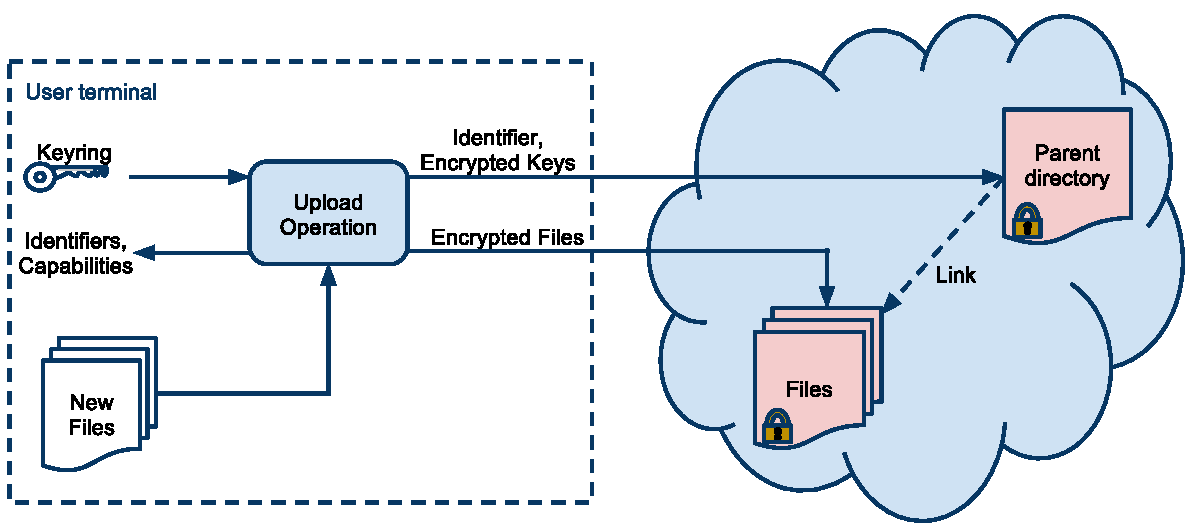
\includegraphics[width=\columnwidth]{ArchitectureUpload.pdf}
%    \caption{Scenario: Uploading of files}
%    \label{fig:arch:upload}
%\end{figure}


\subsection{Generating Keys and Capabilities}

\subsection{Write File to Folder}

\subsection{Encrypt and Upload Folder}

\subsection{Encrypt and Upload File}

\section{Download File}

\section{Share File}
{
-Confidentiality: AES-CBC, RSA

-Integrity: SHA-256

-Authentication: RSA PrK signature

-Key hierarchy

-Key distribution
}

%**************************************%
\chapter{Implementation}
%**************************************%

%**************************************%
\chapter{Results}
%**************************************%

%**************************************%
\chapter{Discussion}
%**************************************%

- Cascading deletes? Loops.

%**************************************%
\chapter{Conclusion and Future Work}
%**************************************%

% BibTeX bibliography lives in external file
\bibliographystyle{plainnat}
\bibliography{references}
% TODO: Can we fix references in order of apperance?

\appendix
\appendixpage
\addappheadtotoc
% Appendix goes here


\end{document}
